\section{Zielsetzung}
\label{sec:Zielsetzung}
\nocite{anleitungV203}
Das Ziel des Versuchs ist die Verdampfungswärme von Wasser zu ermitteln. Hierfür wird Wasser erhitzt und
die Temperatur sowie der Dampfdruck gemessen.

\section{Theorie}
\label{sec:Theorie}
Wasser kann in drei verschiedenen Phasen bzw. Aggregatzuständen fest, flüssig und gasförmig vorliegen.
Diese Zustände sind von dem Druck $p$ und der Temperatur $T$ abhängig. In der Abbildung (\ref{fig:ZustandsdiagrammWasser})
ist die Temperatur- sowie die Druckabhängigkeit des Wasserzustands qualitativ abgebildet.
\begin{figure}[H]
    \centering
    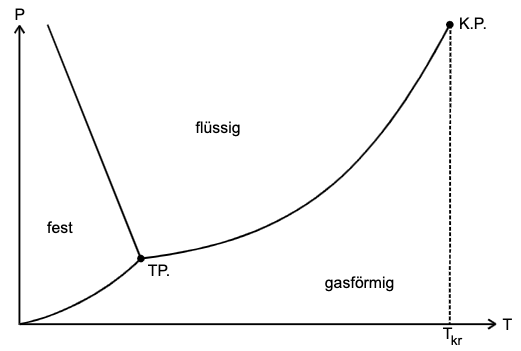
\includegraphics[width=0.95\textwidth]{ZustandsdiagrammWasser.png}
    \caption{Qualitatives Zustandsdiagramm von Wasser. \cite{anleitungV203}}
    \label{fig:ZustandsdiagrammWasser}
\end{figure}
Innerhalb der drei abgeschlossenen Bereichen, welche den drei genannten Phasen von Wasser entsprechen, besitzt das System 
zwei Freiheitsgrade $p$ und $T$. Dahingegen besitzt das System nur einen Freheitsgrad, wenn sich den Grenzlinien angenähert wird. An diesen
Grenzlinien koexistieren zwei Phasen. Am Tripelpunkt (TP.) befindet sich das Wasser im festen, flüssigen als auch im gasförmigen Zustand.
An dem kritischen Punkt koexisiteren die flüssige und gasförmige Phase. 
Die Grenzlinie, die den Tripelpunkt und den kritischen Punkt verbindet, wird Dampfdruckkurve genannt. Dabei wird die Dampfdruckkurve
durch die Verdampfungswärme $L$ charakterisiert. 
\begin{figure}[H]
    \centering
    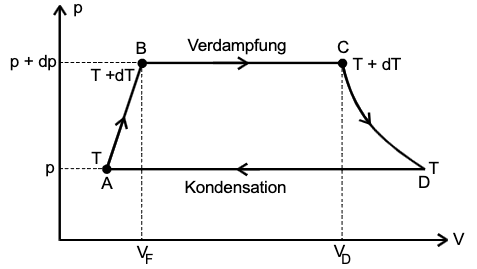
\includegraphics[width=0.95\textwidth]{Kreisprozess.png}
    \caption{Kreisprozess von Wasser in einem p-V-Diagramm. \cite{anleitungV203}}
    \label{fig:Kreisprozess}
\end{figure}
% \subsection{Vorbereitungsaufgaben}
% \label{sec:Vorbereitungsaufgaben}
